\chapter{Método de trabajo}
\label{chap:metodo}

\drop{E}{n} este capítulo se describe la metodología de desarrollo aplicada, sus ventajas y motivo de elección. También se presenta la evolución del proyecto en base a la metodología empleada, los hitos conseguidos en cada fase, su complejidad y el tiempo empleado en cada una de ellas, detallando las iteraciones realizadas hasta conseguir la versión final del sistema.

Para finalizar, se listan y describen todas las herramientas utilizadas en el desarrollo, ya sean hardware o software.
%Igualmente se aportará información del rendimiento (profiling) del sistema en diferentes situaciones.

\section{Metodología del desarrollo}
Para la construcción de un proyecto de cierta envergadura, como es el caso de un Trabajo Fin de Grado, la aplicación de un marco de trabajo para estructurar, planificar y controlar el proceso, es esencial para desarrollar software de calidad.

Las características del proyecto, con requisitos con posibilidad de cambios y adaptaciones a lo largo de todo el proceso, el reducido «equipo de desarrollo» o la necesidad de obtener versiones incrementales que sean testeadas y validadas por el director de proyecto, hacen que la elección se decante hacia \textbf{metodologías ágiles} de desarrollo de software.

Las \textbf{metodologías ágiles} \cite{Ubeda}, utilizan prácticas adaptativas (no basadas en predicciones), iterativas, centradas en personas (clientes y desarrolladores), orientadas a entregas incrementales, con mucha comunicación y  necesitan que el cliente esté muy involucrado en el proyecto para recibir su \textit{feedback}. El \textit{feedback} continuo es indispensable para evitar que el cliente, con el software acabado, diga \textit{«es lo que pedí, pero no es lo que necesitaba»}, algo habitual cuando se utilizan métodos clásicos.

En resumen, las principales características a las que deben dar forma las metodologías ágiles son:
\begin{itemize}
\item \textbf{Incremental:} Versiones pequeñas de software, con ciclos rápidos. 
\item \textbf{Cooperativa:} Desarrolladores y cliente siempre en contacto constante.
\item \textbf{Directa:} El método es fácil de aprender, modificar y está bien documentado.
\item \textbf{Adaptativa:} Son capaces de tolerar los cambios propuestos por el cliente.
\end{itemize}
%Hay que tener en consideración la muy diferente naturaleza de los métodos ágiles. Mientras que Scrum se decanta por la gestión, otros como XP especifican las prácticas a seguir en el equipo, Pragmatic Programming da pautas para desarrollar un buen código, algunos como FDD no abarcan la totalidad del proceso de desarrollo, AgileUP surge como una versión ágil de RUP y propone EUP que es una ampliación para abarcar todo el ciclo de vida del software, etc.
\section{\textit{Scrum}}
\textit{Scrum} ~\cite{Ubeda} está desarrollado para gestionar el proceso de desarrollo de sistemas aplicando ideas de flexibilidad, adaptabilidad y productividad. Sin llegar a describir ninguna técnica de desarrollo de software específica, el objetivo es definir cómo deben funcionar los miembros del equipo para que el sistema sea flexible y se adapte a condiciones altamente cambiantes.
 
\begin{figure}[t] 
  \centering
  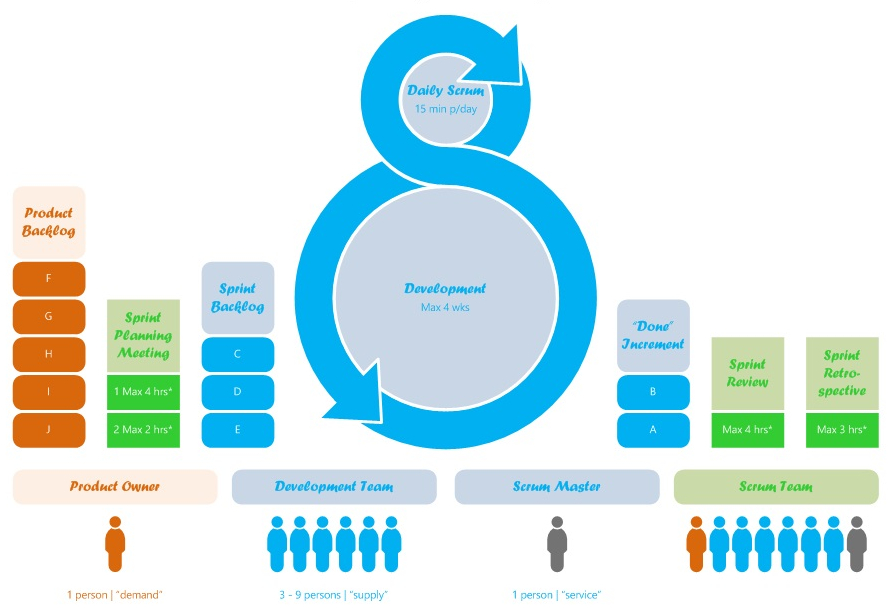
\includegraphics[width=1.0\textwidth]{scrum-overview.jpg}
  \caption{Esquema de trabajo con \textit{Scrum}. (Mark Hoogveld)}
  \label{fig:scrum}
\end{figure}

\subsection{Fases de \textit{Scrum}}
El proceso de \textit{Scrum} consta de tres fases según Schwaber y Beedle \cite{Schwaber}: \textit{Pre-Game}, Desarrollo o \textit{Game} y \textit{Post-game}. La fase \textit{Pre-Game} incluye dos subfases:

\begin{itemize}
\item \textbf{\textit{Pre-game}}
  \begin{itemize} 
  \item El \textbf{\textbf{planning}} incluye la definición del sistema a desarrollar y asegurar la financiación. Se crea una lista ó pila de producto, \textit{Product Backlog List} que contiene todos los requisitos conocidos. Estos requisitos pueden ser añadidos por el cliente, los programadores o incluso otras personas relacionadas con el proyecto. Se priorizan los requisitos y se estima el esfuerzo necesario para su desarrollo. El \textit{planning} también incluye la definición del equipo del proyecto, herramientas, valoración de riesgos y necesidades de formación. 
  \item En la fase de \textbf{arquitectura}, se crea el diseño del sistema a alto nivel basándose en los requisitos actuales del \textit{Backlog}. En el caso de una mejora a un sistema ya existente, se identifican los cambios necesarios, así como los problemas que puedan surgir.
  \end{itemize}
  
\item \textbf{\textit{Game:}} Esta fase se trata como una caja negra donde se espera  que ocurra lo imprevisible. Las diferentes variables técnicas y de entorno que pueden cambiar (calendario, calidad, requisitos, recursos, tecnologías, herramientas, e incluso métodos de desarrollo) se observan y controlan durante los \textit{sprints}. En lugar de considerar estos puntos sólo al principio del proyecto, \textit{Scrum} los controla constantemente para adaptarse a los cambios.
  
  Para la fase de desarrollo, \textit{Scrum} funciona mediante lo que denomina \textit{sprints}. Los \textit{sprints} son ciclos iterativos donde se desarrollan o mejoran las funcionalidades para producir los nuevos incrementos. Cada \textit{sprint} incluye las fases habituales de desarrollo del software: requisitos, análisis, diseño, desarrollo y entrega. Los \textit{sprint} suelen tener una duración entre una semana a un mes.
  
\item\textbf{\textit{Post-game:}} Contiene el cierre de la versión. Se entra en esta fase cuando se completan todos los requisitos. La \textit{release} ya está lista para lanzarse. Es en esta fase donde se integra, prueba y documenta.
\end{itemize}

\subsection{Roles y responsabilidades}
Los papeles desempeñados en \textit{Scrum} tienen tareas y propósitos diferentes durante el proceso y sus prácticas.

\begin{itemize}
\item \textbf{\textit{Scrum Master.}} Es responsable de asegurar que el proyecto se realiza según las prácticas, valores y reglas de \textit{Scrum} y que progresa como estaba previsto. Actúa recíprocamente tanto con el equipo del proyecto como con el cliente. %También es responsable de resolver cualquier impedimento para seguir trabajando tan productivamente como sea posible. 

\item \textbf{\textit{Product Owner.}} El propietario del producto \textit{(Product Owner)} es oficialmente responsable del proyecto.  Gestiona, controla, y administra el \textit{Product Backlog List}. Toma las últimas decisiones de las tareas, participa estimando el esfuerzo de desarrollo para los puntos del \textit{Backlog} y los concreta en funcionalidades a desarrollar.

\item \textbf{Equipo de \textit{Scrum.}} El equipo de \textit{Scrum} tiene autoridad para decidir las acciones pertinentes para organizarse y lograr lo propuesto en cada \textit{sprint}. El equipo de \textit{Scrum} está involucrado en la estimación del esfuerzo requerido para cada parte e identificar problemas a tratar.

\item \textbf{Cliente.} El cliente participa en las tareas relacionadas con los puntos del \textit{Backlog} para diseñar o mejorar el sistema.

%\item \textbf{Director} La gestión o dirección toma la última decisión y se encarga de los documentos, normas y convenciones seguidas en el proyecto. La dirección también participa en identificar objetivos y requisitos. Por ejemplo, ayuda a seleccionar el \textit{product owner}, valorar los progresos y reducir el \textit{Backlog} con el \textit{Scrum Master}.
\end{itemize}

\subsection{Artefactos}
\subsubsection{Documentos}
\begin{itemize}
\item \textbf{\textit{Product Backlog.}} El \textit{Product Backlog} define todo lo necesario en el producto final, basándose en los conocimientos de ese momento. Por tanto, define el trabajo que se tiene que realizar en el proyecto. Incluye una lista ordenada por prioridades y actualizada de requisitos técnicos para que se realice en  el sistema o mejore. 

Los elementos del \textit{Product Backlog}, pueden incluir características, funciones, parches para \textit{bugs}, defectos, peticiones de mejoras o actualizaciones.
 
También se incluyen temas que requieren solución para poder hacer otros puntos de la lista. A la lista de \textit{Backlog} puede contribuir el cliente, el equipo del proyecto y otras personas relacionadas con el proyecto.

\item \textbf{Sprint Backlog.} Es el punto de partida de cada \textit{sprint}. Es una selección de historias del \textit{Product Backlog List} que se llevarán a cabo en el próximo \textit{sprint}. El equipo de \textit{Scrum} junto con el \textit{Scrum Master} y el \textit{Product Owner} seleccionan los puntos basándose en la prioridad y los objetivos. A diferencia del \textit{Product Backlog}, el \textit{Sprint Backlog} no se modifica hasta que el \textit{sprint} termina.
 
Cuando todos los puntos del \textit{Sprint Backlog} se han completado, se prepara una nueva iteración del sistema. El registro que se utiliza el seguimiento, incluye valores que representan las horas de trabajo pendiente, y en función de esos valores se elabora un gráfico denominado \textit{burndown}.

\begin{figure}[h] 
  \centering
  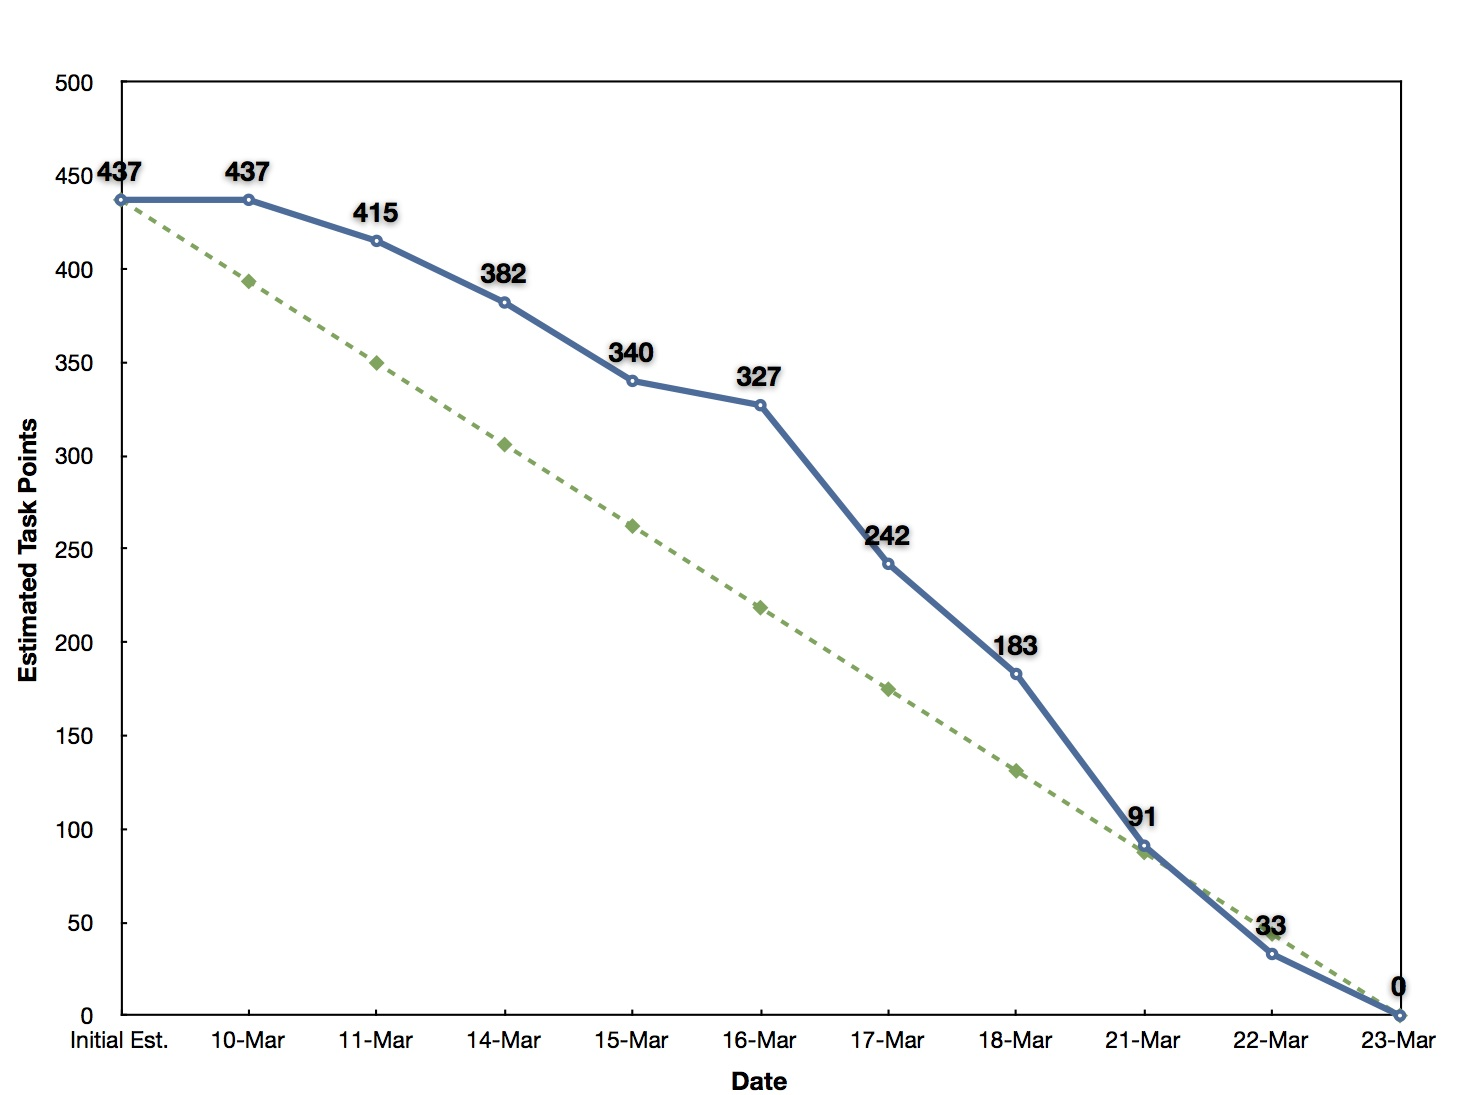
\includegraphics[width=0.85\textwidth]{burndown.jpg}
  \caption{Gráfico \textit{burndown} de un \textit{sprint}}
  \label{fig:burndown}
\end{figure}

\end{itemize}

\subsubsection{Reuniones}
\begin{itemize}
\item \textbf{Reunión diaria de \textit{Scrum}.} Se organizan reuniones de \textit{Scrum} diarias para seguir el progreso del equipo, qué se ha hecho desde la última reunión y qué se hará para la siguiente. También se exponen problemas y otros asuntos que puedan aparecer, se busca y soluciona cualquier deficiencia o imprevisto del proceso.  La duración de estas reuniones es de unos 15 minutos. El \textit{Scrum Master} se encarga de dirigirlas y normalmente se suelen realizar de pie para evitar que puedan alargarse. También se valora la puntualidad de los asistentes; si alguien llega tarde, se le cobra una multa simbólica. 

\item \textbf{Reunión para plantear el \textit{Sprint}.} El \textit{sprint planning meeting} está organizado por el \textit{Scrum Master}, y es donde se eligen los objetivos y las funcionalidades del próximo \textit{sprint}. A continuación, el \textit{Scrum Master} y el equipo concretan la manera de conseguir estos objetivos, lo que se denomina, \textit{(product increment)}, en el siguiente \textit{sprint}.

\item \textbf{\textit{Sprint Review Meeting}.} En el último día del \textit{sprint}, el equipo y el \textit{Scrum Master} presentan los resultados del \textit{sprint} a la dirección, clientes, usuarios y \textit{Product Owner} en una reunión informal. Los participantes evalúan la evolución y deciden sobre las siguientes actividades. 
\end{itemize}

\subsection{\textit{Sprint}}
Un \textit{sprint} consiste en un ciclo iterativo donde se realiza un incremento del sistema. Está dirigido para adaptarse a las condiciones cambiantes del proyecto como requisitos, tiempo, recursos, conocimiento, tecnología, etc. 

El equipo de \textit{Scrum} se auto-organiza para producir el nuevo incremento ejecutable en aproximadamente un mes natural, que suele ser la duración habitual del \textit{sprint}. Las herramientas activas del equipo son las reuniones para planear el \textit{sprint}, el \textit{sprint backlog} y las reuniones diarias de \textit{Scrum}.

\section{\textit{eXtreme Programming}}
\textit{Extreme Programming}  o programación extrema, surgió como respuesta a la lentitud de los modelos tradicionales de desarrollo. Los orígenes de esta metodología surgieron en 1996, cuando Kent Beck comenzó a trabajar en un proyecto para reemplazar el programa de nóminas para Chrysler. Aunque las tácticas por separado que utiliza \textit{XP} no son novedosas, la manera de unirlas sí. 

En la primera edición de \textit{XP} (1999), Beck definió 4 valores, 15 principios básicos, y 12 prácticas. Posteriormente el proceso fue revisado y se publicó en 2004 \cite{Beck:2004:EPE:1076267}, en él se detallan 5 valores, 14 principios, 13 prácticas primarias y 11 prácticas secundarias.

\subsection{Valores}
\begin{itemize}
\item La mayoría de los problemas y errores provienen de la falta de comunicación. Debe haber \textbf{\textit{comunicación}} entre los miembros del equipo y entre el equipo y los clientes. La comunicación más eficaz es la comunicación directa, interpersonal. También los artefactos deben ser fácilmente entendibles y estar actualizados.

\item «Haz lo más sencillo que podría funcionar». Programar de forma sencilla, que no simplista, requiere experiencia, ideas y trabajo duro. La \textbf{\textit{simplicidad}} favorece la comunicación, reduce la cantidad de código y mejora la calidad. La idea subyacente es que las nuevas funciones se podrán agregar cuando se necesiten si el sistema es simple.

\item Siempre debería poder compararse lo que está programado con lo que se quiere programar, respecto a las funciones que se necesiten. El \textbf{\textit{feedback}} lo proporciona el contacto con el cliente y la disponibilidad de pruebas automatizadas que se desarrollan con el propio proyecto. Cuanto más simple es un sistema, más fácil es conseguir \textit{feedback} sobre él. 

\item \textbf{\textit{Valentía}}. Todos los métodos y procesos son herramientas para combatir y reducir nuestros miedos. Cuanto más miedo tengamos a un proyecto de software, mayores y más pesados serán los métodos que necesitaremos. La comunicación, la simplicidad y el \textit{feedback} permiten adaptarse a los cambios grandes en los requisitos. También hay que tener valor para desechar código obsoleto.

\item Los cuatro valores anteriores implican un quinto: el \textbf{\textit{respeto}} entre los miembros y por su trabajo.
\end{itemize}

Los cinco valores no dan consejos específicos sobre cómo gestionar un proyecto, o cómo 
escribir código. Para este propósito, se utilizan las prácticas que se detallan a continuación.

\subsection{Prácticas fundamentales}
\subsection{Análisis de requisitos y Planning}
\begin{itemize}
\item Se describen todas las funciones del sistema usando \textbf{historias}, descripciones breves de funciones que el cliente podrá ver.
\item El desarrollo del software se realiza \textbf{semanalmente}. Hay una reunión al principio de cada semana donde el cliente elige, según prioridades y teniendo en consideración el tiempo necesario por los programadores, las historias a programar durante la semana.
\item \textbf{Evitar hacer promesas} que no puedan cumplirse. 
\end{itemize}

\subsection{Equipo y Factores Humanos}
\begin{itemize}
\item Los equipos de desarrollo deben trabajar en un \textbf{espacio sin divisiones} para facilitar la comunicación.
\item El equipo debe componerse de \textbf{miembros con todas las habilidades necesarias} para el proyecto, sentido de compañerismo y de ayuda mutua. 
\item \textbf{Programación por parejas.} El código siempre está escrito por dos programadores en una única máquina.
\end{itemize}

\subsection{Diseño}
\begin{itemize}
\item \textbf{Diseño Incremental.} \textit{XP} se opone a un gran diseño completo inicial. El equipo escribe código lo antes posible para obtener \textit{feedback} y mejorar el sistema continuamente. La pregunta es cuándo diseñar. \textit{XP} sugiere hacerlo incrementalmente durante la programación.
\item \textbf{Primero las pruebas.} Antes de actualizar y añadir código, es necesario escribir las pruebas para verificarlo. 
\end{itemize}
\subsection{Programar y lanzar versiones}
\begin{itemize}
\item \textbf{La compilación y las pruebas automáticas deben poder finalizar en diez minutos} para ejecutarlo a menudo y obtener \textit{feedback}. 
\item \textbf{Integración continua.} Los programadores deben integrar los cambios cada dos horas para evitar problemas mayores al integrar grandes partes.
\item \textbf{El código y las pruebas son los únicos artefactos que se deben guardar.} Los otros documentos pueden generarse a partir del código y las pruebas.
\item Cualquier miembro del equipo debe tener \textbf{acceso a todas los elementos de sistema} cuando quiera. 
\item \textbf{Sólo hay una versión oficial de sistema.} Se puede desarrollar una rama temporal, pero sólo usarse durante unas horas.
\item \textbf{Despliegue diario.} Al finalizar la jornada se debe poner nuevo software en producción. Es arriesgado y costoso tener diferentes versiones en producción y desarrollo.
\end{itemize}

\section{Aplicación de la metodología de desarrollo}

Para la resolución de este proyecto se ha optado por una aproximación en la que se complementan las mejores prácticas y técnicas recomendadas en \textbf{\textit{Scrum}}, con sus medidas organizativas como método de gestión y \textbf{\textit{extreme programming (XP)}}, con patrones de diseño y refactorización, como metodología de desarrollo.

%Scrum no requiere o proporciona ninguna práctica específica para el desarrollo del software. Sin embargo, se adoptarán las siguientes pautas y prácticas para evitar el caos causado por imprevistos y complejidades.
Se adoptarán las siguientes pautas y prácticas de \textbf{\textit{Scrum}} a la hora de gestionar el proceso de desarrollo:
\begin{itemize}
\item \textbf{Equipo autodirigido} y auto-organizado. 
\item Una vez elegida una tarea, \textbf{no se agrega trabajo extra}. %En caso que se agregue algo, se recomienda quitar alguna otra cosa.
\item \textbf{Iteraciones de 30 días}; se admite que sean más frecuentes.
\item \textbf{Demostración a participantes externos} al final de cada iteración. 
\item Al principio de cada iteración, \textbf{planificación adaptativa} guiada por el director.
\end{itemize}

El  equipo  de  desarrollo  lo  han constituido el autor de este TFG y Santiago Sánchez Sobrino, con  experiencia  práctica y conocimientos teóricos en metodologías ágiles. Debido  al  tamaño  del  equipo  y  condiciones  del  mismo,  las  reuniones  diarias pierden su utilidad. La figura del cliente y el director corresponde a Carlos González Morcillo, director de ambos TFG's y creador del \textit{Proyecto ARgos}. 

Al comienzo de cada iteración el equipo se reunirá y creará la lista de tareas de la iteración (\textit{Sprint Backlog}) que consta de un subconjunto de las \textit{historias de usuario} de la lista de objetivos (\textit{Product Backlog}). Estas historias de usuario son seleccionadas atendiendo a las prioridades o necesidades propuestas por el Director. En esta reunión, se descompondrá cada historia en tareas, estimando el tiempo necesario para llevarlas acabo. 

Las prácticas propuestas de \textbf{\textit{XP}} que se van a utilizar son: 

\begin{itemize}
\item \textbf{Sentarse juntos.} Todo el desarrollo se llevará a cabo en un espacio que permita un trabajo cercano, cooperativo y que facilite la comunicación directa. %En las ocasiones en las que esto no sea posible, se utilizarán medios de videoconferencia como Skype o Hangouts. 

\item \textbf{Iteraciones cortas.}  Al trabajar con pequeñas iteraciones, se obtiene el \textit{feedback} del cliente con mucha frecuencia. Con esto se pretende que el producto final cubra ampliamente sus expectativas y necesidades. 

\item \textbf{Integración continua.} No se utilizarán herramientas que automaticen este proceso, no obstante, debido al tamaño reducido del equipo y a la frecuencia de las integraciones (al menos una al día), esta tarea no resultará demasiado compleja. 

\item \textbf{Diseño incremental.} A pesar de definir buena parte de la arquitectura en las primeras iteraciones, el diseño del sistema evolucionará iteración tras iteración, sometiéndose a sucesivas refactorizaciones para mejorar su calidad.  

\item \textbf{Código compartido.} Todos los miembros del equipo podrán acceder a cualquier parte del código. Sin olvidar que el presente desarrollo ágil se encuentra en el contexto de la elaboración de PFCs y que los alcances deben estar acotados para cada uno de los alumnos. Al finalizar cada  iteración se destinará tiempo a completar y refinar la documentación obtenida del proceso.

\item \textbf{Reutilización del código} Uno de los principales objetivos que se persiguen con las metodologías ágiles es entregar proyectos en tiempo y bajo presupuesto, minimizando el \textit{Time To Market}, por lo que la reutilización del código constituye un aspecto muy importante, no se ha de perder tiempo \textit{«reinventando la rueda»} en cada proyecto. Se deben obtener diseños con una alta modularidad y lo más desacoplados posibles, reutilizando como cajas negras, los elementos software que necesitemos. 

%Se ha de tener en cuenta que no todos los elementos en un proyecto son reutilizables, puesto que es inevitable que algunos estén estrechamente ligados a condiciones particulares propias de cada dominio de aplicación, la modularidad tampoco ha de convertirse en una obsesión que obstaculice el avance del proyecto. Recordemos que si se conoce la mejor forma de hacer algo, que así se haga, sino que se haga de la mejor forma conocida para la que se tenga tiempo. 
\end{itemize}

\section{Evolución del proyecto}
Esta sección describe los cambios ocurridos en el proyecto según su planificación prevista. En cada una de las iteraciones, se exponen los objetos que se pretenden obtener y la toma de decisiones ocurrida en el proceso.

%\subsection{Concepto del software}

\subsection{Análisis preliminar de requisitos}
El objetivo de este proyecto es construir un sistema de ayuda a la gestión de documental que permita el tratamiento directo sobre documentos físicos impresos mediante el uso de técnicas de visión por computador, síntesis visual y auditiva y técnicas de realidad aumentada.

Los requisitos para el sistema serán proporcionados por Carlos González Morcillo, creador e investigador principal del proyecto; la cátedra Indra-UCLM y la fundación Adecco, como financiadores del proyecto y la Asociación ASPRONA, que con su experiencia en la atención a personas con discapacidad, propondrán escenarios y funcionalidades que sean de utilidad para este colectivo. 

\subsubsection{Características de los usuarios}
Aunque el usuario final del sistema, será cualquier persona que necesite soporte en la gestión documental de documentos impresos, el fin de esté proyecto es construir un sistema que permita la integración laboral a personas con discapacidad. 

El tipo de usuarios a los que estará dirigido son, en primer lugar, personas que pueden presentar un amplio espectro de discapacidades. El sistema debe proporcionar soporte a usuarios con discapacidades sensoriales (visuales y auditivas) e intelectuales.  

\subsubsection{Restricciones}
Debido a los objetivos del sistema, se deben tener en cuenta las siguiente restricciones:
\begin{itemize}
\item\textbf{Funcional en dispositivos móviles.} El prototipo final se construirá sobre un dispositivos con arquitectura ARM con limitaciones de tanto en capacidad de computo como memoria. El sistema deberá estar optimizado para este tipo de dispositivos, obteniendo una respuesta fluida y en tiempo real.   
  
\item\textbf{Se debe basar en componentes de bajo coste.} Para facilitar la implantación real en el entorno de trabajo, deberá funcionar con componentes de bajo coste, incorporando mecanismos de corrección de distorsión y registro 3D totalmente software.
\end{itemize}

\subsubsection{Interfaces Hardware}
\begin{itemize}
\item La implementación del sistema se realizará sobre una Raspberry Pi Modelo B de 512MB de RAM y arquitectura ARM. 
\item La visualización será a través de un pico-proyector mediante conexión HDMI.
\item El acceso al sistema y conexión a internet se establece por medio de cable ethernet durante el desarrollo y pruebas, siendo la conexión WiFi el tipo de conectividad final.
\end{itemize}

\subsubsection{Requisitos funcionales}
\paragraph{Definidos en la línea base del proyecto}
\begin{itemize}
\item RF-001: Adquisición de imágenes mediante cámara USB.
\item RF-002: Adquisición de imágenes mediante raspiCam.
\item RF-003: Sistema de calibrado de cámaras y proyectores.
\item RF-004: Configuración del sistema mediante argumentos por terminal.
\item RF-005: Implementación de una interfaz natural de usuario.
\item RF-006: Control Gestual.
\item RF-007: Identificación rápida de documentos.
\item RF-008: Sistema de cálculo de homografías.
\end{itemize}

\paragraph{Definidos por ASPRONA}
\begin{itemize}
\item RFa-001: Realización de Videoconferencias.
\item RFa-002: Mensajes en Lectura Fácil.
\item RFa-003: Soporte para completar partes de trabajo.
\item RFa-004: Soporte para completar formularios de protocolos de calidad.
\item RFa-005: Guiado para clasificación y archivado de facturas.
\item RFa-006: Entorno configurable por el usuario.
\end{itemize}
%\paragraph{Definidos por Indra/Adecco}
%\begin{itemize}
%\item RFi-001: Reconocimiento de Firmas
%\end{itemize}
\subsubsection{Requisitos no funcionales}

\begin{itemize}
\item\textbf{Rendimiento:} El sistema debe funcionar de manera fluida y en tiempo real en dispositivos móviles basados en arquitectura ARM. Sólo existirá un único usuario del sistema simultáneamente y los documentos a tratar también se tratarán de uno en uno.

\item\textbf{Seguridad:} A parte de la información que se proporcione al usuario directamente, se mantendrá un \textit{log} donde se registrará toda la actividad realizada en el sistema.
Debido al carácter experimental del proyecto, no se tendrán en cuenta la aplicación, por lo menos en la primera fases de desarrollo, de técnicas criptográficas para ficheros, bases de datos o comunicaciones.

\item\textbf{Fiabilidad:} Todo tipo de incidente producido en el sistema debe ser controlado y tratado. 

\item\textbf{Disponibilidad:} La disponibilidad del sistema debe ser de al menos un 99\% del tiempo que esté en ejecución. En caso de caída del sistema se deben proporcionar mecanismos automáticos para que la maquina y el sistema se reinicien y sean nuevamente operativos sin la necesidad de intervención directa del usuario,

\item\textbf{Mantenibilidad:} El desarrollo en un dispositivo tan reciente implica que se liberen con relativa frecuencia bibliotecas o controladores, en los que se corrigen \textit{bugs} y/o mejoran su rendimiento. Seria recomendable hacer una revisión de los módulos actualizados antes de la instalación del sistema para valorar si es relevante el beneficio que aportan y no comprometer el la estabilidad del sistema.  

\item\textbf{Portabilidad:} El desarrollo se  realizará siguiendo estándares, tecnologías y bibliotecas libres multiplataforma, con el objetivo de que pueda ser utilizado en el mayor número de plataformas posibles tanto software como hardware.
\end{itemize}

\subsubsection{Otros requisitos}
La distribución del proyecto se realizará mediante alguna licencia libre como GPLv3, para ello se utilizarán bibliotecas compatibles con dicha licencia.

\subsection{Revisión sistemática de la bibliografía}
Como punto de partida para la elaboración del estado del arte se realizo una revisión sistemática de las diferentes técnicas para la identificación de documentos y su recuperación de una base de datos. Como resultado de esta revisión se ha podido conocer las técnicas más empleadas, así como sus ventajas e inconvenientes. 

El claro ganador es LLAH (Locally Likely Arrangement Hashing) con casi un 40\% de utilización ya sea con su implementación inicial o implementaciones optimizadas creadas para salvar las limitaciones del algoritmo original, lo que lo hace aún más potente y versátil.

Aunque los métodos basados en detección de descriptores de características invariantes como SIFT, SURF, aparecen como muy utilizados, realmente no funcionan correctamente en identificación de documentos ya que no presentan zonas de textura y se producen repeticiones de patrones binarios (el propio texto cumple este patrón). La mayoría son una variación del proceso inspirado en la metodología de Lowe [SIFT], y en la que se obtienen buenos resultados sobre documentos semi-estructurados realizando una selección de puntos extraídos y una adaptación del algoritmo RANSAC para la validación de supuestos aciertos en la comparación. 

El algoritmo tiene una tasa elevada de recuperación y precisión, es robusto a las deformaciones que pueda tener la imagen (perspectiva) y no necesita ningún paso previo de segmentación pero, como inconvenientes, no funciona ante grandes secciones de texto y la identificación que realiza es para obtener documentos similares (un ticket, un billete de tren,....) a la imagen utilizada como consulta.

Uno de los puntos del análisis de resultados, indica que al utilizar hardware con distinto rendimiento, es difícil tener mediciones normalizadas para todos los métodos. Como trabajo futuro se puede realizar la implementación de varios de los métodos más utilizados, y ofrecer un estudio comparativo completo al ejecutarse sobre una misma plataforma.

%Existen varias implementaciones optimizadas sobre LLAH para salvar las limitaciones iniciales del algoritmo. Sería un trabajo futuro la tarea de buscar sólo las publicaciones que se hayan hecho sobre LLAH e intentar crear una implementación conjunta  con todas las optimizaciones. 
\subsection{Diseño general}
El diseño de GrayAR, se ha abordado con la idea principal de construir un \textit{framework} de realidad aumentada completamente modular y extensible. Para ello, se realizó una clasificación de funcionalidades organizada en módulos y submódulos, siendo cada uno de ellos lo más independiente posible del resto y de las bibliotecas en las que se basaban. Entre las \textit{«herramientas de diseño»} aplicadas para conseguir estos objetivos, se encuentran los patrones de diseño software, que nos proporcionan catálogos de elementos reusables, y la solución estándar y óptima a problemas ya conocidos y solucionados anteriormente.

Esto puede ocasionar un aumento de la complejidad, pero definiendo una arquitectura orientada a componentes, permite la ampliación de la funcionalidad de forma sencilla, la posibilidad de realizar optimizaciones concretas o incluso, la reescritura completa de un módulo, sin que ello afecte en el resto de la plataforma. 

\subsection{Iteraciones}

\subsubsection{Iteración 0}
La iteración 0, se puede considerar la fase anterior al inicio del proyecto. El tiempo empleado en esta iteración comprendió entre el 18 de noviembre de 2013 y el 12 de diciembre de 2013.

Con la idea general del proyecto definida, se adquieren un par de Raspberry Pi y se realiza una búsqueda de pico-proyectores candidatos para utilizar. El proyector debe tener un precio ajustado, ser lo más reducido posible, y además, tener una luminosidad suficiente para que las proyecciones sean visibles en estancias iluminadas.  

Una vez recibida la Raspberry Pi, se procede a la configuración del entorno de trabajo. Este proceso incluye la instalación del sistema operativo Raspbian, la biblioteca OpenCV, compiladores, editores y la configuración del servicio de SSH para poder controlar la Raspberry desde el puesto de trabajo.

En esta iteración, se inicia la búsqueda y recopilación de \textit{papers} para la elaboración del estado del arte, el aprendizaje de la biblioteca OpenCV para adquirir una base de conocimientos en el área de la visión por computador, y un estudio de fundamentos matemáticos en álgebra lineal y geometría proyectiva.

Finalmente, el 10 de diciembre de 2013, se mantuvo una reunión con los miembros de la asociación ASPRONA para explicarles los objetivos del proyecto y obtener de ellos, un escenario de casos de uso basados en la experiencia que tienen en la inserción laboral de personas con discapacidad. Estos casos de uso, se transformó en una especificación de requisitos para nuestro sistema.

\subsubsection{Iteración 1}
La realización de la construcción y pruebas de esta iteración, se llevó a acabo entre el 12 de diciembre de 2013 y el 8 de enero de 2014.

Las limitadas capacidades de la Raspberry Pi y la experiencia que otros programadores han tenido a la hora de trabajar en sistemas de visión por computador en este dispositivo, nos pone en alerta de que es posible, llegado un momento, la alta carga de computo que tienen los procesos de visión por computador afecten al rendimiento y perdamos la sensación de tiempo real. Las consecuencias de esto, es que sea necesario que los procesos más costosos deban ser ejecutados en otro dispositivo o computador con mejores prestaciones.  

Partiendo de las premisas anteriores, no queda otra opción de realizar una arquitectura completamente modular y con todos los subsistemas desacoplados. Una clase \emph{core} será la encargada de inicializar todos los subsistemas, establecer las comunicaciones entre ellos y ejecutar la lógica de usuario soportada dentro de un bucle infinito.

El objetivo de esta primera iteración es obtener una arquitectura básica que iremos completando y refinando en cada una de las sucesivas iteraciones. Se decide que el \textit{sprint} abarque la construcción y pruebas de las siguientes \textit{historias}:

\paragraph{Captura de imágenes.}
La Raspberry tiene la opción de conectar cámaras USB. Se construye un módulo de captura de vídeo, utilizando las funciones de la clase \texttt{VideoCapture} de OpenCV, que proporciona los distintos frames necesarios para dar soporte al resto de módulos del sistema. 

Para la medida de rendimiento se implementa el cálculo de los FPS que da el sistema a la salida y que nos va a determinar si se obtienen resultados aceptables para un sistema de tiempo real. Los primeros resultados son mucho peores de lo esperado. A una resolución de 320x240 píxeles y sólo realizando el proceso de captura y visualización de los frames capturados en pantalla, se observa un lag de 2 segundos y una tasa de 2 FPS. 

Si estos valores son inadmisibles en un sistema en tiempo real con una arquitectura tan básica, y sin realizar ningún tipo de procesado en la imagen, cuando se deba realizar algún tratamiento a la imagen o computo adicional, el sistema no será usable, con una sensación de bloqueo del sistema para el usuario.

Se vuelven a realizar las pruebas con otra cámara USB más moderna (Logitech S720) y afortunadamente los resultados mejoran sensiblemente, a 6 FPS y hasta 10 FPS para imágenes obtenidas en blanco y negro.  
   
\paragraph{Detección de una hoja de papel.}
Mediante segmentación de la imagen obtenida, se detecta una hoja de papel y se obtiene la posición de sus 4 esquinas en píxeles de pantalla. Esta funcionalidad se encapsula dentro de la clase \texttt{PaperDetector}
Durante las primera fase de pruebas nos pone en situación de los numerosos factores que influyen en este tipo de sistemas. El primero de ellos es la iluminación. El tipo de luz (natural, fluorescente, incandescente,...), intensidad de la luz natural (luz por la mañana, al mediodia o por la tarde), dirección de la luz (crea sombras en uno u otro sentido), los reflejos producidos por las superficies se convierten en interferencias en forma de grandes manchas en la imagen. Incluso se han detectado variaciones en la detección al encontrase varias personas entre el sistema y una ventana.
 
\subsubsection{Iteración 2}
Los objetivos de esta iteración venian condicionados por los malos resultados obtenidos en el \textit{sprint} anterior. Hay que conseguir mejorar enormente los resultados anteriores o la viabilidad del proyecto se verá seriamente afectada. Se estableció la duración de la iteración entre el 8 de enero y el 3 de febrero.  

\paragraph{Optimización de la captura de imágenes.}
Durante las pruebas de la iteración anterior, con sólo cambiar la cámara USB se obtuvieron grandes mejoras, por lo que la elección de la cámara era un elemento importante. Tras consultar en diversos foros especializados, se decide que la mejor opción es utilizar la \textbf{\textit{Raspberry Pi Camera Board}}. Esta cámara está especialmente diseñada para utilizarse en la Raspberry, y se conecta directamente al conector CSI de la placa mediante un cable plano flexible de 15 pines. Dispone de un sensor de 5MP de resolución y puede llegar a grabar vídeo a 1080p a 30 fps.

El gran inconveniente de es que la cámara no incluye drivers \textit{video4linux}, por lo que cualquier biblioteca para lectura de cámaras web estándar, OpenCV incluido, no es capaz de obtener los frames producidos. 

Con la cámara se proporcionan 2 aplicaciones: \texttt{raspivid} y \texttt{raspistill}, para la captura de vídeo e imágenes respectivamente. Las aplicaciones utiliza la API MMAL (Multi-Media Abstraction Layer), para acceder a los datos de la cámara y transferirlos a la pantalla o codificarlo como imágenes o vídeos. A partir del código fuente disponible de estas aplicaciones, Pierre Raufast modificó el código fuente, para que una vez obtenidos los datos de la cámara, utilizar el \textit{buffer} de memoria para construir estructuras de tipo \texttt{CvMat} propias de OpenCV.

Partiendo del trabajo de Pierre, otras personas, como Chris Cummings o Rafael Muñoz Salinas, están construyendo bibliotecas en C++ para poder obtener las imágenes de la cámara en objetos compatibles con OpenCV. Es precisamente la biblioteca de Rafael Muñoz, la que se ha utilizado a modo de drivers. 

Tras sustituir el módulo de captura con la nueva biblioteca para la \textit{Raspberry Camera Board}, se realizan de nuevo los test de rendimiento, y obtenemos casi 30 PFS, que es un buen resultado para aplicaciones en tiempo real.

\paragraph{Calibrado de la cámara.}
Se construye un programa externo para el calibrado de la cámara basado en un patrón de tablero de ajedrez. Esta primera versión, devuelve un fichero XML con los parámetros intrínsecos de la cámara y los coeficientes de distorsión obtenidos, pero no tiene en cuenta el error de reproyección.

\paragraph{Sistema básico de cálculo de homografías.} 
En esta primera fase, los cálculos son los necesarios para realizar el registro y visualizarlo en la pantalla del ordenador. Dentro del proyecto, se crea la clase \texttt{CameraModel} encargada de leer los ficheros de calibración y almacenar los parámetros propios de la cámara que serán utilizados para el cálculo de los parámetros extrínsecos. 

Para el cálculo y almacenamiento de la posición de los folios respecto a la cámara se construye la clase \texttt{Paper}.

Las pruebas realizadas al módulo de cálculo de la posición y rotación del papel, son satisfactorias, y se puede comprobar que el dibujado de ejes de coordenadas, o distintos poliedros en el espacio 3D es correcto y perfectamente alineado con el papel. 

\paragraph{Dibujado mediante OpenCV.}
En la iteración anterior se realizaron una serie de funciones auxiliares para dibujado de contornos, puntos y polígonos mediante OpenCV que sirviesen de soporte para el \textit{«modo debug»}. Para la iteración actual, estas funciones se ha aumentado con dibujado de ejes de coordenadas, cubos y ortoedros para validar los cálculos de la posición y rotación de los folios. También permite recibir una ventana con la imagen por medio de SSH. Con todas estas funciones se ha creado la clase estática \texttt{DrawCV}. 

\subsubsection{Iteración 3}
El siguiente paso es incorporar el proyector al sistema. Acoplando la Raspberry Pi sobre el proyector y colocando la raspiCam junto a la lente obtenemos un conjunto compacto y reducido. El sistema se monta sobre un trípode y se coloca en dirección a la mesa.

Los objetivos son, por tanto, obtener un sistema de calibrado. Debido a la complejidad de la tarea, se establece como la única tarea a realizar en este \textit{sprint}.

Aunque el \textit{sprint} inicialmente se planteo con una duración aproximada de un mes, la construcción y las numerosas pruebas realizadas para garantizar el correcto funcionamiento finalmente se llevaron a cabo en cerca de dos meses, del 3 de febrero de 2014 al 31 Marzo de 2014. 

\paragraph{Calibrado del sistema cámara-proyector}
Un proyector se calibra usando los mismos algoritmos que una cámara ya que puede considerarse como una \textit{«cámara invertida»}. Sin embargo como el proyector no ve, y el método no es tan directo como en el caso de una cámara. Además es necesario realizar los cálculos para la transformación entre el sistema de referencia de la cámara y el sistema de referencia del proyector.

El estudio de distintas técnicas de calibrado nos llevó a considerar dos procedimientos. El primero, siguiendo el enfoque de Zhang, en el se utilizan patrones planos, y el propuesto por Daniel Moreno y Gabriel Taubin, basado luz estructurada.

Aunque según los \textit{papers} consultados, el método basado en luz estructurada, es más preciso que otras técnicas de calibrado, el procedimiento es más costoso de realizar. El método de Zhang, permite un procedimiento más flexible, no necesita una preparación exhaustiva de la escena y tiene una precisión aceptable para los objetivos de nuestro proyecto.

Con el código para el calibrado de cámaras de la iteración anterior, realizamos una ampliación para añadir la funcionalidad del calibrado del proyector.

Para calibrar el proyector, es necesario obtener un conjunto de coordenadas 3D-2D correspondientes. Las coordenadas se determinan utilizando la cámara situada en una posición con una vista similar a la que tendría el proyector. El método consiste en realizar una proyección de un plano de calibrado y establecer la correspondencia entre lo proyectado y lo que ve la cámara.
 
Ahora dispondremos de los puntos 3D en el sistema de referencia global (el patrón), y también su proyección (puntos 2D en la imagen) en el sistema de referencia de la cámara y en el sistema de referencia del proyector. 

Finalmente, aplicando un procedimiento de calibrado estéreo como el que proporciona OpenCV obtenemos la transformación entre la cámara y el proyector.

El resultado, con los parámetros intrínsecos y extrínsecos, se escribe en ficheros YAML para cargarlos en el sistema. Mientras que la cámara y el proyector mantengan su posición y rotación entre ellos, no es necesario realizar una nueva calibración y es posible mover todo el sistema.  

Entre las decisiones tomadas en este \textit{sprint}, fue realizar el calibrado como una aplicación externa al sistema. Esto nos permite la reutilización del módulo para otros sistemas estéreo.

Otras decisión fue la resolución de imagen con la que trabajaría el sistema. El proyector tiene una resolución nativa de 854x480 en formato 16:9, pero la Raspberry Pi no la soporta. Se eligió una resolución de 1280x720, pero con este tamaño de imagen, el rendimiento disminuía significativamente. También se utilizó 800x600 en formato 16:9, pero la distorsión que realizaba el proyector para mostrar la imagen en formato panorámico no podíamos medirla para realizar una corrección, y los puntos calculados no correspondían con los objetos situados sobre la mesa.

La resolución que se estableció finalmente fue de 800x600 en formato 4:3. Se perdía algo de superficie de proyección, pero con aumentar un poco la distancia entre el proyector y la mesa se compensaba esta área, y además, el rendimiento del sistema con esta resolución era adecuado y entraba dentro de los parámetros para un sistema de tiempo real.

\subsubsection{Iteración 4}
El periodo de la iteración transcurrió entre el 31 Marzo de 2014 y el 28 de Abril de 2014. 

Desde la iteración 2, se arrastraba un pequeño \textit{bug} en el cálculo de los parámetros extrínsecos del papel. Entre los objetivos planificados en esta iteración se decidió que también se corrigiese este bug, quedando finalmente el \textit{sprint backlog} con los siguientes elementos:

\paragraph{Corrección de la orientación del papel}
En el cálculo de los parámetros extrínsecos del papel, dependiendo de la posición del papel, el sistema confundía la orientación y consideraba que el papel se encontraba apaisado cuando realmente no era así.

La corrección del \textit{bug} fue relativamente sencilla. Tras una serie de pruebas rotando la hoja de papel para comprobar en que casos se producía el error, se observó que el problema era debido a como OpenCV enumerar las esquinas del papel. Dado un cuadrilátero, la primera esquina corresponde a la que se encuentra situada más a la derecha de la imagen. Cómo se puede observar en la figura [X], en el primer caso el punto $A$ es enumerado como punto $0$, y sin embargo, en la segunda imagen es considerado el punto $1$. 

Las consecuencias son que para ciertas posiciones, las dimensiones de los segmentos que forman los lados del papel tienen un valor, y en otras posiciones, esos mismos segmentos tienen otra medida. En resumen, para el cálculo de los parámetros extrínsecos, considera una distribución distinta en entre los puntos de la imagen y los puntos del objeto.

La solución implementada ha sido comparar la longitud de los segmentos detectados, para determinar en que posición se están enumerando las esquinas, y aplicar una enumeración acorde al establecido en los puntos del objeto. 
 
\paragraph{Detector de documentos mediante descriptores de imágenes} 
Se eligió utilizar SURF como detector y descriptor de características debido que es más rápido y robusto que otros algoritmos. Aun así, la implementación de esté modulo se realizó utilizando los \textit{wrappers} que proporciona OpenCV para la construcción de detectores y descriptores, y que tiene como ventaja, cambiar el algoritmo aplicado sin necesidad de modificar la implementación, únicamente modificando en el constructor un \textit{string} con el método que queramos utilizar (BRISK, ORB, SURF,...).

\paragraph{Optical Flow}
Para la estimación y descripción del movimiento, se implementó \textit{Optical Flow} (Lucas-Kanade) que proporciona herramientas para detección, segmentación y seguimiento de la hoja de papel en la escena a partir de un conjunto de imágenes. En etapas posteriores, debido a la oclusión que se realiza sobre el papel, se decidió que no cumplía las expectativas como metodo de tracking y se rechazó. 

\subsubsection{Iteración 5}
A estas alturas del desarrollo del proyecto, la carga de trabajo que debe soportar la Raspberry Pi es muy significativa. Se aprecia que el rendimiento se ve afectado al incluir la detección de documentos, ya que es una tarea costosa para el sistema, y aun queda por implementar el módulo de interacción natural, que se trata también de una tarea con gran carga de trabajo.

Durante la reunión de planificación, se acuerda que se realicen las siguientes tareas en el periodo del 28 de Abril de 2014 al 12 de Mayo de 2014:

\paragraph{Migración del sistema al servidor}
Como ya se venía observando, en cada iteración el rendimiento general del sistema en la Raspberry era cada vez menor. No sólo tenia que soportar los módulos de GrayAR, sino que también debía soportar la ejecución de \textit{BelfegAR}. El objetivo de la iteración anterior de \textit{Belfegar}, fue crear una arquitectura cliente-servidor que permitiese la delegación de tareas entre la Raspberry Pi y un servidor. Este servidor, seria el encargado de realizar la ejecución de los módulos más costosos del sistema y descargar a la Raspberry Pi, para realizar las tareas de captura y representación más holgadamente.

Gracias a que se tuvo en cuenta que este caso pudiese ocurrir, y la decisión temprana construir un sistema  modular y desacoplado, la migración al servidor y la conexión mediante la unidad de delegación de tareas de \textit{Belfegar} fue prácticamente transparente y sin realizar modificaciones en los módulos creados.

Aprovechando esta arquitectura, también se separó el programa de calibración, lo que supuso una reducción considerable del tiempo empleado para realizar el calibrado del sistema cámara-proyector.
 
\paragraph{Implementación de un histórico de percepciones}
Al igual que en ARToolKit, se desarrolla una función de tratamiento del histórico de percepciones para estabilizar el \textit{tracking}. Este histórico se implementa almacenando las últimas 4 percepciones similares y realizando una media ponderada, en la que las percepciones recientes tienen más peso que las antiguas. Para determinar si son percepciones próximas se establece un umbral. Mediante el uso de esta técnica eliminamos gran parte del efecto tembloroso en la proyección.

\paragraph{Optimización del proceso de detección de rectángulos}
La función para detectar hojas de papel implementada en la iteración 1 es muy básica. No permite que exista ninguna oclusión y es muy sensible a la iluminación. Tras un estudio de técnicas alternativas, se opta por implementar el cálculo de la envoltura convexa del contorno. Además de ser un algoritmo más reducido, la mayor ventaja que aporta este método es que tolera ciertos solapamientos en los bordes del papel. 

Para optimizar más la función, se sustituye el método de binarización de la imagen. Se cambia la umbralización adaptativa por el método de Canny. Con este cambio, se obtiene un algoritmo más robusto, más tolerante a la iluminación y que devuelve bordes más finos, con lo que también aumenta la precisión del sistema.

\subsubsection{Iteración 6}
Esta iteración supone la construcción del sistema de interacción natural de usuario. Al finalizar esta iteración, se podrá realizar acciones sobre los botones que está desarrollando \textit{BelfegAR} y que permitirán ofrecer una experiencia de usuario muy enriquecida al mostrar información opcional a petición del usuario. Para este desarrollo se estimó una duración entre el 12 de Mayo de 2014 y el 23 de Junio de 2014.

\paragraph{Segmentación de manos}
Para extraer el contorno de la mano de la imagen se decide utilizar un filtrado por el color de la piel. Existen numerosos artículos sobre este tema, y todos concluyen que los mejores resultados se obtienen realizando la búsqueda en el espacio de color HSV \textit{(Hue, Saturation, Value)}. Para convertir las imágenes a este espacio de color, es necesario que la captura se realice en color. Hasta esta iteración, la adquisición de imágenes se estaba efectuando en escala de grises, ya que consumía menos recursos, y el color no era una propiedad que necesitásemos.

Teniendo en cuenta que los procesos de cálculo están en el servidor, obtener las imágenes a color no supuso una pérdida de rendimiento en el sistema. Además, con sólo realizar la conversión a escala de grises de la imagen, los métodos
ya implementados y que no necesitan la imagen a color no tienen que ser modificados.

La segmentación implementada, se basa en la selección del los píxeles de la imagen que pertenezcan al rango habitual del color de la piel. Para aumentar la tolerancia del algoritmo, se le aplica a la imagen una serie de filtros, y finalmente se obtiene una máscara con la región de la mano en la imagen.

\paragraph{Cálculo de la posición del dedo}
Una vez obtenida el contorno de la mano, se debe buscar su posición. En un principio se pensó en implementar el reconocimiento de todos los dedos de la mano, pero se optó por sólo reconocer el índice. Esta decisión, vino determinada por la funcionalidad de interacción que se iba a implementar, que era la pulsación de un botón, por lo que examinar la posición del resto de los dedos es, en principio, innecesaria. 

\subsubsection{Iteración 7}
Con el sistema de interacción de usuario funcionando el sistema, se advierte que el módulo de detección de papeles funciona correctamente cuando no hay solapamientos o si la oclusión se encuentra muy próxima a los bordes. En la reunión del \textit{sprint} se considera que se debe implementar una nueva mejora de la detección de papeles, y establece esta iteración entre el 23 de Junio de 2014 y el 14 de Julio de 2014.

\paragraph{Detección de papeles con solapamiento}
Analizando los solapamientos que se realizan sobre el papel en función de las posiciones de la mano, se observa que normalmente quedan visibles partes de los lados del papel. Se decide realizar la búsqueda de segmentos rectos mediante la transformada de Hough y generar las posibles combinaciones de 4 segmentos del conjunto de rectas detectadas. Aquellos que cumplan las restricciones de formar una hoja de papel, serán los posibles candidatos.

Este segundo método de detección es más costoso que el anterior, por lo que se determinó que de forma predeterminada, el sistema utilizase la detección basada en la envoltura convexa cuando no existiesen solapamientos, y en caso de fallo, se aplicase esta nueva función. 

Los resultados de las pruebas fueron muy satisfactorias. Esta nuevo algoritmo detectaba el papel aún existiendo grandes solapamientos, tanto en bordes como en esquinas del documento.

\subsubsection{Iteración 8}
Durante es periodo del 14 de Julio de 2014 al 25 de Agosto de 2014, prácticamente no se efectuaron modificaciones al sistema. Se realizaron algunas correcciones de \textit{bugs} y se ajustaron algunos parámetros en la configuración de los algoritmos de visión por computador. La mayor parte de esta iteración fue destinada a la realización, tanto de la presente memoria, cómo del informe técnico a presentar tras la finalización del \textit{Proyecto ARgos}.

\subsubsection{Iteración 9}
El 15 de Septiembre, recibimos de la Asociación ASPRONA una serie de formularios y partes de trabajo para que se implementase un caso real mediante los documentos que ellos utilizaban habitualmente. Tras una reunión, se establece el nuevo \textit{sprint} entre el 15 de Septiembre de 2014 y el 28 de Noviembre de 2014. Las tareas que se realizan son la preparación y entrenamiento del sistema para adecuarlo a la documentación recibida.
 
Para facilitar el cambio de configuración y no tener que recompilar constantemente, se implementa un gestor de configuración. Este gestor nos permite la modificación de los distintos parámetros del sistema sin la necesidad de recompilar nuevamente el proyecto cada vez que se realiza un cambio. También, de cara a la versión final, se ajustan el sistema para que no sea necesario utilizar una base de fondo negro, que se estuvo utilizando para mejorar el contraste entre papel y mesa.

Con el sistema preparado, definimos el flujo uso de cara a la «demo final» y se graba un vídeo de demostración. 

El 15 de Octubre el proyecto es presentado en el \textbf{5º Congreso Nacional CENTAC de Tecnologías de la Accesibilidad} con gran aceptación por parte del público asistente. Se concertó una reunión el 28 de Octubre con la Asociación ASPRONA, donde tras la demostración, expresaron interés por el sistema y el potencial que tiene para la adaptación y ayuda a personas con discapacidad en el puesto de trabajo.

Finalmente, el 25 de Noviembre de 2014 en otra reunión mantenida, fue expuesto a responsables de Indra y la fundación Adecco.   

\section{Tecnologías y herramientas utilizadas}

En esta sección se listan y detallan los recursos software y hardware empleados en la construcción de la plataforma. Además de una breve explicación del recurso, se enuncia la versión utilizada y sobre qué plataformas opera.

\subsection{Hardware}
\begin{itemize}
\item \textbf{Raspberry Pi.} Se trata de la unidad de detección y despliegue del sistema. En el Anexo~\ref{chap:anexo_caracteristicas_rpi} pueden verse las características oficiales del modelo empleado.
\item \textbf{Raspberry Pi Camera Board}  Se trata de una minicámara de 5MP con un sensor Omnivision 5647, que se conecta directamente a la Raspbery Pi a través de un conector CSI.
\item \textbf{Proyector portátil.} Se trata del medio principal que permite el despliegue de gráficos del sistema. El proyector empleado es un Optoma PK320 que soporta una resolución panorámica máxima de 854x480. 
\item \textbf{Amplificador de Audio} Se trata de un circuito integrado LM386 montado en una placa de test con un altavoz de 1W para proporcionar audio al sistema.
\item \textbf{Tarjeta de memoria:} Se emplea una MicroSDHC Trascend de 32GB clase 10, como unidad de almacenamiento de la Raspberry Pi. Proporciona una velocidad de lectura y escritura de 20 MB/s y 17 MB/s respectivamente. 
\item \textbf{Equipo informático}  Para el desarrollo del proyecto ha sido necesario hacer uso de un computador conectado por red a la plataforma Raspberry Pi, para poder acceder remotamente a ella y de esta forma ejecutar las pruebas. El equipo es un Intel Core i7-2600K 3.4 GHz 4 núcleos y dos hilos por núcleo 16 GB de RAM y Nvidia GeForce GTX 560 Ti.

\end{itemize}

\subsection{Software}
A continuación se enumeran las diversas herramientas software empleadas y diferenciadas por categorías:

\subsubsection{Lenguajes de programación}
\begin{itemize}
\item \textbf{C++} - El lenguaje empleado para el desarrollo del proyecto ha sido C++ \cite{Stroustrup00}, debido a la eficiencia y velocidad de ejecución que proporciona a la hora trabajar en aplicaciones y sistemas en tiempo real. También por ser el estándar referente en bibliotecas gráficas y de visión artificial.
\end{itemize}

\subsubsection{Sistemas Operativos}
\begin{itemize}
\item \textbf{Debian} - Es una distribución de GNU/Linux desarrollada y mantenida por una comunidad de voluntarios. Es una de las famosas y un gran número de distribuciones están basadas en ella. Para el desarrollo del proyecto se ha utilizado la versión \emph{unstable}. 

\item \textbf{Raspbian} - Es una distribución de GNU/Linux basada en Debian Wheeze especialmente diseñada y optimizada para la ejecución en la placa Raspberry Pi con  CPU ARMv6   
\end{itemize}

\subsubsection{Aplicaciones de desarrollo GNU}
\begin{itemize}
\item \textbf{GNU Emacs} - Editor y entorno de desarrollo. Se ha utilizado la generación del código fuente y la escritura de la documentación.  Se han empleado, además, algunos \textit{plugins} como
  ECB~\footnote{\url{http://ecb.sourceforge.net/}}, que añade al editor funcionalidades propias de un entorno
  de desarrollo completo. Versión 24.3.1
\item \textbf{GNU Make} - Herramienta para la compilación incremental, con soporte multiproceso.
\item \textbf{GNU GCC} - La colección de compiladores GNU. En concreto se ha utilizado el compilador de C++ (g++) en su versión 4.5.2.
\item \textbf{GNU GDB} - Se trata del depurador por excelencia de los sistemas GNU/Linux. Se ha utilizado la versión 7.2.
\item \textbf{GNU GPROF} - Es una herramienta para hacer profiling (ver Sección 6.2) para compiladores de la familia gcc. Se ha utilizado la versión 2.21.
\item \textbf{GNU CMAKE} - Se trata de una herramienta análoga a make, aunque de más alto nivel, para la automatización de generación de código. Se ha utilizado principalmente para la compilación de la biblioteca RaspiCam. La versión de CMake es la 2.8.3. 
\end{itemize}

\subsubsection{Documentación y gráficos}
\begin{itemize}
\item \textbf{Doxygen} - Sistema de documentación de código fuente. Compatible con C++.
\item \textbf{InkScape} - Programa de edición de imágenes vectoriales.
\item \textbf{Draw.io} - Servicio web para dibujado de diagramas y gráficos vectoriales..
\item \textbf{GIMP} - Herramienta de manipulación de gráficos.
\item \textbf{LibreOffice Draw} - Potente herramienta de dibujado vectorial perteneciente a la suite ofimática LibreOffice. Utilizada para la generación de diagramas para la documentación. Versión 3.5.4.
\item \textbf{\LaTeX{}} - Es un sistema de composición de textos, orientado especialmente a la creación de libros, documentos científicos y técnicos que contengan fórmulas matemáticas. Elegido para la generación de la documentación mediante la distribución Texlive. 
\item \textbf{AUCTeX} -  Para la elaboración de este documento se ha empleado este paquete~\footnote{\url{http://www.gnu.org/software/auctex/}} que permite integrar las funciones
  de \LaTeX en los menús del editor Emacs.
\item  \textbf{esi-tfg} Clase \LaTeX{} del grupo \acs{ARCO} desarrollada por David Villa, y que proporciona una plantilla con la que se ha maquetado este documento.
\end{itemize}


\subsubsection{Bibliotecas}
\begin{itemize}
\item \textbf{OpenCV} - Biblioteca libre que proporciona funciones dirigidas principalmente para el desarrollo de aplicaciones de visión por computador en tiempo real. La versión utilizada es la 2.4.9
\item \textbf{RapidXML} - Se trata de un intérprete o \textit{parser} para archivos XML.
\item \textbf{RaspiCam} - Es una biblioteca para la utilización de la cámara Raspberry Pi Board desarrollada en C++ por el grupo de investigación «Aplicaciones de la Visión Artificial» de la Universidad de Córdoba. La versión utilizada es la 0.1.1 
\end{itemize}

\subsubsection{Control de Versiones}
\begin{itemize}
\item \textbf{Git} - Sistema de control de versiones distribuido. Como repositorio central se ha utilizado la plataforma Bitbucket.
\end{itemize}
